% WIECON-ECE 2026 conference paper -- corpus/resource-paper revision.
% The corpus, the WLS pipeline, the dual-axis keying, and the failure registry
% are the contributions; the two-model channel study is explicitly illustrative.
\documentclass[conference]{IEEEtran}
\usepackage{amsmath,amssymb,amsfonts}
\usepackage{graphicx}
\usepackage{textcomp}
\usepackage{booktabs}
\usepackage{balance}
\usepackage[colorlinks=true,linkcolor=black,citecolor=black,urlcolor=black]{hyperref}

\setlength{\abovecaptionskip}{3pt}
\setlength{\belowcaptionskip}{1pt}
\setlength{\textfloatsep}{7pt plus 2pt minus 2pt}
\setlength{\floatsep}{7pt plus 2pt minus 2pt}
\setlength{\intextsep}{7pt plus 2pt minus 2pt}

\makeatletter
% force table/figure captions to exactly 8pt (class default is 9pt here)
\long\def\@makecaption#1#2{%
\ifx\@captype\@IEEEtablestring%
\fontsize{8}{9}\selectfont\bgroup\par\centering\@IEEEtabletopskipstrut{\normalfont\fontsize{8}{9}\selectfont #1}\\{\normalfont\fontsize{8}{9}\selectfont\scshape #2}\par\addvspace{0.5\baselineskip}\egroup%
\@IEEEtablecaptionsepspace
\else
\@IEEEfigurecaptionsepspace
\setbox\@tempboxa\hbox{\normalfont\fontsize{8}{9}\selectfont {#1.}\nobreakspace\nobreakspace #2}%
\ifdim \wd\@tempboxa >\hsize%
\setbox\@tempboxa\hbox{\normalfont\fontsize{8}{9}\selectfont {#1.}\nobreakspace\nobreakspace}%
\parbox[t]{\hsize}{\normalfont\fontsize{8}{9}\selectfont\noindent\unhbox\@tempboxa#2}%
\else%
\ifCLASSOPTIONconference \hbox to\hsize{\normalfont\fontsize{8}{9}\selectfont\hfil\box\@tempboxa\hfil}%
\else \hbox to\hsize{\normalfont\fontsize{8}{9}\selectfont\box\@tempboxa\hfil}%
\fi\fi\fi}
\makeatother

\begin{document}

\title{GridPowerAgent: A Seeded, Reproducible Scenario Corpus for Power-System LLM Evaluation}

\markboth{GridPowerAgent: A Seeded, Reproducible Scenario Corpus for Power-System LLM Evaluation}{}

\maketitle
\vspace{-3ex}
\vspace{1ex}

\begin{abstract}
Evaluating large language models (LLMs) on power-system tasks requires observations that reveal what the model actually reads: several recent evaluations feed a plain-language description of the injected disturbance alongside the measurements and report near-perfect diagnosis. We present GridPowerAgent, a seeded, fully regenerable scenario corpus for power-system LLM evaluation: 15,000 scenarios across the IEEE 14, 39, and 118 bus systems, ten injected disturbance classes, 9.54 million correlated measurements, per-scenario iterative weighted-least-squares (WLS) state estimates, dual-axis reference keying, a reproducible 41-scenario failure registry, and an executable pandapower tool back-end. The corpus ships three observation channels that separate what a model reads from what it reasons about: a plain-language event description, EMS-grade telemetry, and raw summary state. An illustrative study---one seeded 140-scenario draw, two models, single temperature-zero runs with exact denominators---demonstrates the corpus's central measurement: description-only diagnosis is 100\%, the description is the answer key; from telemetry alone the API model reaches 93.9\% while a 4-bit local model drops to 43.8\% (20-scenario probe); from raw summary state the API model collapses to 8.0\% while a gradient-boosted classifier on identical features reaches 64.3\%. The corpus, the estimation pipeline, the keying, and the registry are the contribution; the study illustrates what they enable, not a general finding about grid-LLM evaluation.
\end{abstract}

\noindent\textit{Keywords---}benchmark corpus, cause-keyed labels, iterative WLS, LLM evaluation, observation channels, pandapower, power systems, reproducibility, scenario generation, state estimation

\section{Introduction and Related Work}
LLMs are increasingly proposed for power-system operations: reading grid states, classifying disturbances, selecting analysis tools, and advising operators \cite{achiam2023gpt4,majumder2024joule,zhang2025gridagent,wen2025xgridagent}. Evaluating such claims requires a test corpus with three properties that published evaluations---LLM dispatch benchmarks \cite{zhou2024elecbench,cheng2025gaia} and reinforcement-learning grid testbeds \cite{marot2020l2rpn,donnot2020grid2op} alike---rarely provide: the labels are derived by a transparent, reproducible rule system; every scenario carries physical ground truth; and the observation given to the model is separated from the information used to grade it. This paper presents such a corpus and the evaluation harness built around it.

\emph{Why seeded and regenerable matters.} A seeded corpus changes what an evaluation can claim. Fixed draws mean every model, prompt version, and observation channel is scored on byte-identical inputs, so paired comparisons are exact rather than resampled. Regeneration from seeds makes label provenance auditable: every label traces to an injection record and a solver run, and leakage audits (did the observation disclose the label?) are plain joins over the 54 scenario fields. Physical ground truth also enables non-LLM baselines---the classifiers in Sec.~\ref{sec:channels} that bound what information each channel carries---which pure text benchmarks cannot run. Finally, a released corpus turns evaluation into regression testing: new models are scored against prior runs on identical scenarios instead of re-annotated prompts.

Three threads are relevant. \emph{LLM grid evaluations} report strong task performance: ElecBench evaluates dispatch prompting \cite{zhou2024elecbench} and GAIA fine-tunes a dispatch model \cite{cheng2025gaia}; both grade answers to prompts that describe the event in plain language. \emph{Agentic grid systems} couple LLMs to grid environments---Grid-Agent \cite{zhang2025gridagent} for control, X-GridAgent \cite{wen2025xgridagent} for analysis---and report end-to-end system behavior without shipping an evaluation corpus. \emph{Reinforcement-learning testbeds} (L2RPN \cite{marot2020l2rpn}, Grid2Op \cite{donnot2020grid2op}) ship reproducible scenario sets with simulator ground truth, but their interfaces target RL topology control rather than LLM-facing observation channels. Table~\ref{tab:comparison} positions GridPowerAgent against these artifacts: it combines seeded regenerable scenarios, per-scenario physics ground truth, cause-keyed reference labels, separated observation channels, shipped state estimates, and an executable tool back-end in one artifact.

This paper contributes the artifact, not a model ranking. The contributions are: (1) a seeded, fully regenerable corpus of 15,000 scenarios across the IEEE 14, 39, and 118 bus systems (3,000/5,000/7,000; 300--700 per disturbance class), generated from seeded injections over 16,000 operating points, each carrying pre- and post-event power-flow ground truth \cite{wood2014power}, 9.54 million correlated measurements, and physics flags; (2) a per-scenario measurement and iterative-WLS state-estimation pipeline with a disclosed noise model, shipped estimates, and audited accuracy; (3) a dual-axis reference keying that keeps outcome-keyed and cause-keyed labels scoreable side by side, plus a reproducible registry of the 41 IEEE-39 injections that produce unresolvable islands; (4) three separated observation channels with an executable pandapower tool back-end and a closed-loop protocol; and (5) an explicitly illustrative two-model, one-draw study of the observation channels that demonstrates what the corpus measures. The corpus, the estimation pipeline, the keying, and the registry stand on their own; nothing in this paper argues a general claim about grid-LLM performance.

\begin{table}[!t]
\centering
\caption{Released artifacts compared. Seed = reproducible scenario sets; Phys. = per-scenario power-flow ground truth; Obs. = LLM-facing observation channels; Label = cause-keyed reference labels; WLS = shipped iterative-WLS state estimates; Tools = executable pandapower back-end; LLM = LLM performance reported. --- = not part of the released artifact.}
\label{tab:comparison}
\fontsize{7}{8}\selectfont
\setlength{\tabcolsep}{3.5pt}
\begin{tabular}{|l|c|c|c|c|c|c|c|}
\hline
\textbf{Artifact} & \textbf{Seed} & \textbf{Phys.} & \textbf{Obs.} & \textbf{Label} & \textbf{WLS} & \textbf{Tools} & \textbf{LLM} \\ \hline
ElecBench \cite{zhou2024elecbench} & -- & -- & -- & -- & -- & -- & $\checkmark$ \\ \hline
GAIA \cite{cheng2025gaia} & -- & -- & -- & -- & -- & -- & $\checkmark$ \\ \hline
Grid-Agent \cite{zhang2025gridagent} & -- & -- & -- & -- & -- & -- & $\checkmark$ \\ \hline
X-GridAgent \cite{wen2025xgridagent} & -- & -- & -- & -- & -- & -- & $\checkmark$ \\ \hline
L2RPN \cite{marot2020l2rpn} & $\checkmark$ & $\checkmark$ & -- & -- & -- & -- & -- \\ \hline
Grid2Op \cite{donnot2020grid2op} & $\checkmark$ & $\checkmark$ & -- & -- & -- & -- & -- \\ \hline
GridPowerAgent (ours) & $\checkmark$ & $\checkmark$ & $\checkmark$ & $\checkmark$ & $\checkmark$ & $\checkmark$ & $\checkmark$ \\ \hline
\end{tabular}
\end{table}

\section{The GridPowerAgent Corpus}
\label{sec:corpus}
Fig.~\ref{fig:methodology} overviews the generation pipeline. Networks use pandapower \cite{thurner2018pandapower} IEEE 14/39/118 cases \cite{zimmerman2011matpower} with tuned thermal limits to make compound events observable (14: 3\% line / 4\% transformer; 118: 6\%; 39: nameplate). Limits are disclosed per system and deliberately \emph{not} comparable across systems. Operating points sweep load $0.70$--$1.10\times$ with $\pm5\%$ bus-local noise, renewable fractions, and storage state of charge $0.15$--$0.85$ (20 MW/40 MWh at bus 9 on IEEE-14). Topology hashes pin all three networks. Ten classes are injected: E0 Normal; E1 load surge, E2 load drop, E3 line outage, E4 generator outage, E5 renewable ramp (cause classes); E6 undervoltage, E7 overvoltage, E8 thermal overload (outcome classes, physically iterated to target severity); E9 compound.

\begin{figure}[!t]
\centering

\includegraphics[width=\columnwidth]{figs/fig_methodology_tree.png}
\caption{Corpus generation pipeline (stages 03--28).}
\label{fig:methodology}
\end{figure}

\subsection{Composition}
Table~\ref{tab:corpus} summarizes the corpus. Scenarios inject the ten classes with 300/500/700 per class on 14/39/118; replay over 40 draws confirms exact determinism. Fig.~\ref{fig:composition} shows the class composition of the three systems.

\emph{Scenario anatomy.} Every scenario row is self-describing (54 fields). For example, IEEE14\_SCN\_000901 (E3, transmission-line outage) draws operating point IEEE14\_OP\_002268 (load scale 0.77, 194.9~MW system load), injects a \texttt{line\_outage} on target \texttt{line\_6\_12}, and records matched pre/post quantities: minimum voltage 0.9865$\to$0.9851~pu at bus 14, with no resulting limit violations on this draw. Injection descriptors (mechanism, scope, targets, magnitude), the operating point, post-event power-flow quantities, violation counts and flags, and per-quantity deltas all ship in one row, so labeling, subsetting, and leakage audits are plain joins.

Under the cause-keyed default, class counts shift from the 300-per-class injection design because the E6/E8 scenarios re-key to the mechanism that produced them: the IEEE-14 labels are 300 each for E0--E2, E5, and E7; 579 for E3; 329 for E4; and 592 for E9.

\begin{table}[!t]
\centering
\caption{Corpus summary per system.}
\label{tab:corpus}
\fontsize{7}{8}\selectfont
\begin{tabular}{|l|c|c|c|c|}
\hline
\textbf{Case} & \textbf{OPs} & \textbf{Scenarios} & \textbf{Per class} & \textbf{Measurements} \\ \hline
14 (ref) & 4k & 3,000 & 300 & 361k \\ \hline
39 & 5k & 5,000 & 500 & 1.50M \\ \hline
118 & 7k & 7,000 & 700 & 7.68M \\ \hline
\end{tabular}
\end{table}

\subsection{Severity Ladders and Compound Design}
The cause classes (E1--E5, E9) inject a mechanism and record whatever state results. The outcome classes are built the opposite way: a physical disturbance is applied, the power flow is solved, and the outcome is \emph{detected}---if the disturbance did not produce the target state, the scenario is escalated along a severity ladder or discarded, so for every E6/E8 scenario the solver, not the author, decided the voltage or loading. This is also why E7 is generated through reactive mechanisms (excitation set-point shifts rather than load/renewable manipulation): on the stiff IEEE-14 system, injections cannot lift the bus-voltage maximum above 1.05~pu at all (the measured ceiling is 1.0347~pu at minimum load with both renewables at 100\% and the battery discharging). Compound scenarios apply exactly two component mechanisms in order and record the union of their targets. The measured severity envelope on IEEE-14 bounds the corpus: every single-line outage converges and none islands the system, the worst branch loading reaches 228\% (line\_1\_2 outage), and the deepest voltage sag reaches 0.9425~pu (line\_9\_14 outage).

\subsection{Measurements and Iterative WLS State Estimation}
Each scenario carries a fixed meter complement generated from the noise-free power-flow solution: 118 meters per IEEE-14 scenario (14 bus-voltage magnitudes with $\sigma_V=0.003$~pu, 76 branch-end P/Q, 28 bus injections), 301 per IEEE-39 scenario, and 1{,}098 per IEEE-118 scenario---9.54 million readings corpus-wide. Branch-end and injection meters both use $\sigma_P=\max(0.0075|S_{\text{true}}|, 0.05)$~MVA, and every reading ships its true value, noisy measurement, $\sigma$, and standardized $z$-score. The state estimate supplied to the agent is produced by an \emph{iterative AC-WLS estimator} \cite{abur2004power,monticelli1999state} (\texttt{pandapower.estimation}) over these measurements, with branch meters of outaged elements excluded: the estimator converges on 140/140 pilot scenarios with voltage RMSE 0.0064~pu against post-event truth, and the under-voltage flag agrees with truth in 75\% of scenarios---marginal violations can vanish under estimation, which the closed-loop evaluation in Sec.~\ref{sec:closedloop} probes directly.

\subsection{Failure Registry}
Two IEEE-39 switching injections disconnect load pockets and produce unresolvable islands (41 scenarios, NaN post-event voltages). Their identifiers and causes ship with the corpus (case39\_nan\_scenarios.csv) and the scenarios are excluded from evaluation; the resolution plan is an islanding-aware contingency pre-filter in the next corpus revision. Table~\ref{tab:registry} lists the registry in full.

\begin{table}[!t]
\centering
\caption{Islanding failure registry (IEEE-39, 41 scenarios, excluded from evaluation).}
\label{tab:registry}
\fontsize{7}{8}\selectfont
\begin{tabular}{|l|l|c|}
\hline
\textbf{Switched element} & \textbf{Islanded buses} & \textbf{Scenarios} \\ \hline
line\_16\_19 & 19, 20, 33, 34 & 24 \\ \hline
line\_23\_36 & 36 & 17 \\ \hline
\multicolumn{2}{|l|}{Total} & 41 \\ \hline
\end{tabular}
\end{table}

\subsection{Dual-Axis Reference Keying}
\label{sec:dualaxis}
Every scenario ships two label versions: the original v1 keying labeled the two outcome classes (E6 undervoltage, E8 thermal overload) by post-event outcome, and the revised v2 keying labels every scenario by its injected mechanism. The outcome information remains in the per-scenario physics flags, so both axes stay scoreable. The v1 keying proved consequential---models graded under it scored zero on E6/E8 while describing the injecting cause correctly---so the cause-keyed version is the evaluation default, and the failure mode is reproducible by design rather than latent.

\subsection{Artifact Inventory and Reproducibility}
Per system, the released artifact contains the scenario table (CSV and JSONL), pre/post power-flow ground truth, the full measurement set with true value, noisy measurement, $\sigma$, and $z$-score per meter, the WLS state estimates for the pilot draws, both reference-label axes, and the islanding registry; the tool back-end, the FAISS knowledge base, and all run CSVs ship alongside. Networks are pinned by topology hash, operating points and injections are seeded draws, and 40-draw replay reproduces the scenarios byte-identically. Regeneration requires only pandapower and the seeded generation scripts; no number in this paper depends on unreleased data.

\begin{figure}[!t]
\centering
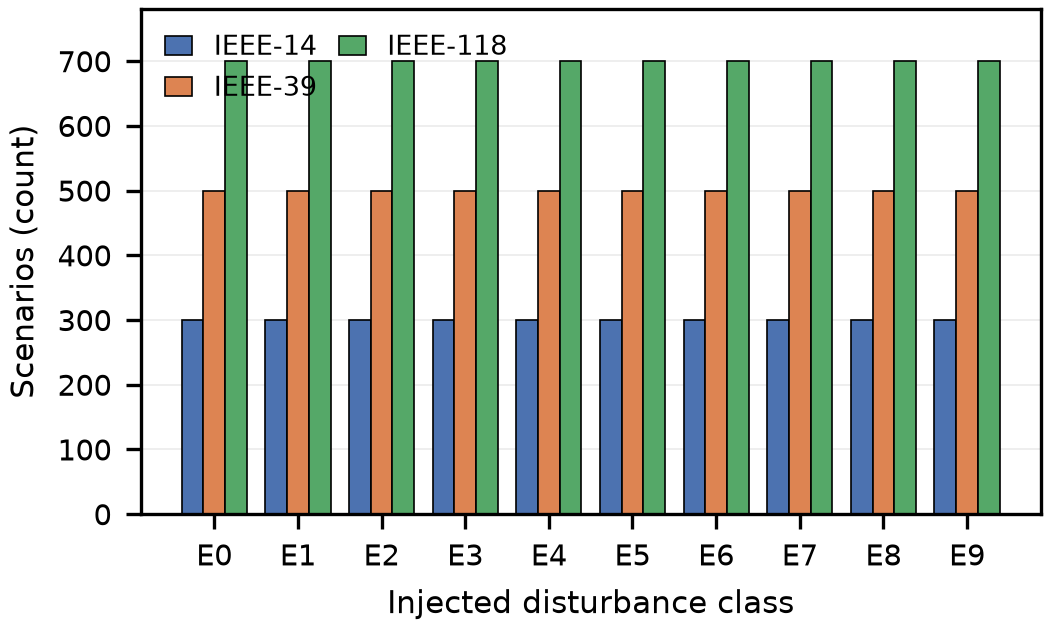
\includegraphics[width=\columnwidth]{figs/fig_corpus_composition.png}
\caption{Class composition of the three systems (scenarios per injected class).}
\label{fig:composition}
\end{figure}

\subsection{Tools and Knowledge Base}
A pandapower back-end exposes five executable operations: full AC power flow, N-1 contingency testing on a named branch, OPF \cite{frank2012opf}, and grid queries (topology, limits, equipment). A retrieval-augmented knowledge base \cite{lewis2020rag}: FAISS \cite{johnson2021faiss} chunks eight operational documents (thermal/voltage limits, contingency procedure, storage/equipment, topology) into 384-d sentence-transformer embeddings \cite{reimers2019sentencebert}, retrieving $k=3$ chunks with citations.

\subsection{Using the Corpus}
The generation choices imply an evaluation protocol. Score against the cause-keyed axis and report which axis was used: the outcome-keyed variant ships so that the keying failure of Sec.~\ref{sec:dualaxis} is reproducible by design rather than latent. Report the observation channel with every number: the three channels are separate prompt-side payloads over byte-identical scenarios, so channel and model effects never have to be disentangled after the fact. Prefer paired seeded draws: regression-testing a new model against prior runs on identical inputs makes comparisons exact rather than resampled. Exclude the 41 registry scenarios (or handle islands explicitly)---their identifiers ship with the corpus. Run non-LLM classifier baselines on each channel before interpreting model scores: a channel that no classifier can separate cannot be expected to inform any model. In closed-loop use, grade element construction separately from class match: the two coincide on single-mechanism events and part on compounds (Sec.~\ref{sec:closedloop}).

\section{Evaluation Harness}
\label{sec:design}

\textbf{Prompt contract and configurations.} The prompt contract is fixed across all studies: the system prompt fixes the persona and tool rules, the user message carries the observation-channel payload, and the answer must be a JSON object naming the diagnosis class---and, in the closed-loop condition, the switched element. Four tool configurations ship with the harness---E1 bare prompt, E2 with retrieved knowledge-base chunks, E3 with executable tools, E4 with both---so retrieval and tool effects can be ablated under an identical contract; retrieval-augmented configurations append the $k=3$ retrieved chunks with citations to the user message.

\textbf{Observation channels.} Three prompt-side conditions probe what diagnosis measures: \emph{description-only} (the plain-language event statement, no grid numbers), \emph{telemetry} (an observed-evidence block with no event statement), and \emph{full} (both). The telemetry block is fixed and fully disclosed---five lines: which branches are open and which generators are offline (by element name); which demand elements changed; which renewable elements changed; system-wide pre$\to$post deltas for load, slack generation, and losses; and deltas for $V_\mathrm{min}$, $V_\mathrm{max}$, and peak loading. It contains observable facts only: no injected intent, no natural-language description. A WLS-estimated variant of the telemetry channel replaces the true post-event values in this block with estimated ones. Table~\ref{tab:telemetry} shows the complete block for the case-study scenario of Sec.~\ref{sec:casestudy}: the demand-side component is fully legible here (eleven changed demand elements, $\Delta$load $+40.28$~MW)---exactly the information the closed-loop status table omits.

\begin{table}[!t]
\centering
\caption{The complete telemetry block for scenario IEEE14\_SCN\_002945 (cause-keyed class E9, the case study of Sec.~\ref{sec:casestudy}). This is the full payload: no description, no injected intent.}
\label{tab:telemetry}
\fontsize{7}{8}\selectfont
\begin{tabular}{|p{0.93\columnwidth}|}
\hline
Switching: branches OPEN: line\_3\_4; no generators offline \\ \hline
Changed demand elements: load\_bus\_2, load\_bus\_3, load\_bus\_4, load\_bus\_5, load\_bus\_6, load\_bus\_9, load\_bus\_10, load\_bus\_11, load\_bus\_12, load\_bus\_13, load\_bus\_14 \\ \hline
Changed renewable elements: none \\ \hline
$\Delta$ load: $+40.28$~MW; $\Delta$ slack generation: $+45.77$~MW; $\Delta$ losses: $+5.49$~MW \\ \hline
$\Delta V_\mathrm{min}$: $-0.0118$~pu; $\Delta V_\mathrm{max}$: $+0.0000$~pu; $\Delta$ peak loading: $+0.357$~pp \\ \hline
\end{tabular}
\end{table}

\textbf{Models.} The illustrative study of Sec.~\ref{sec:results} runs two models under this contract: a lightweight API model (Gemini 3.5 Flash Lite, temperature 0, $\le 512$ output tokens) and a small 4-bit-quantized open-weight model \cite{dettmers2023fourbit,frantar2023gptq} (Gemma 4 E4B-it \cite{gemma4_2026}, served locally from a GGUF build \cite{llamacpp}; temperature 0, $\le 1{,}024$ tokens, reasoning channel parsed with content priority). The API tier is deliberately lightweight: the study characterizes a local deployment against a budget API tier, not against frontier models.

\textbf{Closed-loop tool protocol.} The closed-loop condition embeds the agent in a tool loop in the reasoning-plus-acting \cite{yao2023react} and tool-calling \cite{schick2023toolformer} style: it proposes structured calls with arguments, each call is validated against the network (referenced elements must exist) and executed by the real pandapower back-end, returned measurements re-enter the conversation, at least two executed calls are required before an answer is accepted, and the answer must name the switched element. The closed-loop observation differs from the one-shot telemetry block: the agent sees a per-element status table (each branch as \emph{name $|$ in-service $|$ loading \%}, each generator as \emph{name $|$ offline state}) and, from tools, system summaries (voltage extremes, peak loading, overload list)---switching state and loading, but no demand-side deltas.

\textbf{Metrics.} Diagnosis correctness is exact class match against the cause-keyed reference; tool-call validity requires referenced elements to exist and calls to execute; closed-loop episodes additionally receive a construction grade (did the answer name the true switched element). For paired designs the harness reports the minimum detectable difference (MDE) at $\alpha=0.05$, power 0.80, $(z_{0.975}+z_{0.80})\sqrt{p_\mathrm{d}/n}$, where $p_\mathrm{d}$ is the paired discordance rate. All study numbers are exploratory single temperature-zero runs with exact denominators.

\section{Illustrative Study}
\label{sec:results}
This section demonstrates what the corpus measures; it does not establish a model ranking. Scope: one seeded draw of 140 scenarios per condition (20 for the local telemetry probe), the two models of Sec.~\ref{sec:design}, single temperature-zero runs with exact denominators. We read the numbers as evidence about the corpus's instruments---that its channels separate description-reading from state-based diagnosis---not as findings about model classes.

\subsection{Observation Channels and Baselines}
\label{sec:channels}
With only the plain-language event description available, the API model diagnoses 100.0\% (560 scenarios): reading the description is sufficient, confirming that the description functions as an answer key when present. Table~\ref{tab:channels} and Fig.~\ref{fig:channels} report diagnosis by channel. From telemetry alone the API model reaches 93.9\%; replacing the true post-event state with the WLS estimate leaves it at 97.1\%. From raw summary state it collapses to 8.0\%, answering E7 for most scenarios. The signal exists: a gradient-boosted classifier on identical features reaches 64.3\% from raw state and 100.0\% from telemetry, so the raw-state shortfall is an encoding limit, not an information limit---exactly the distinction the corpus is built to expose. The local model shows the same logic from the other side: 96.8\% with description+state, 43.8\% from telemetry alone (20-scenario probe); the two readings separate only under the realistic channel. Because the channels are prompt-side payloads scored on byte-identical draws, every number above is exactly paired: the corpus makes the observation channel a first-class reported variable by construction rather than by discipline.

\begin{figure}[!t]
\centering
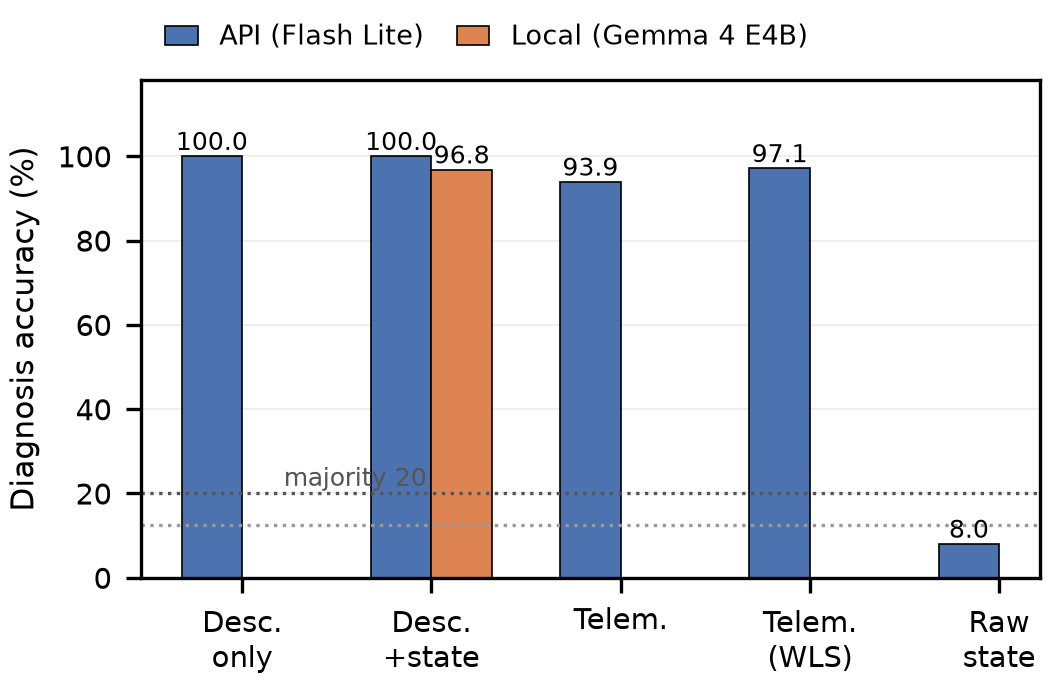
\includegraphics[width=\columnwidth]{figs/fig_observation_channels.png}
\caption{Illustrative study: diagnosis by observation channel and tier (one seed draw, two models). Dotted lines: majority (20.0\%) and random (12.5\%) baselines.}
\label{fig:channels}
\end{figure}

\begin{table}[!t]
\centering
\caption{Illustrative study: diagnosis accuracy (\%) by observation condition. Classifiers fitted on non-pilot scenarios, evaluated on the pilot draw.}
\label{tab:channels}
\fontsize{7}{8}\selectfont
\begin{tabular}{|l|c|c|c|}
\hline
\textbf{Condition} & \textbf{API} & \textbf{Local} & \textbf{GBM} \\ \hline
Description only & 100.0 & -- & -- \\ \hline
Description + state & 100.0 & 96.8 & -- \\ \hline
Telemetry & 93.9 & -- & 100.0 \\ \hline
Telemetry (WLS est.) & 97.1 & -- & -- \\ \hline
Raw state only & 8.0 & -- & 64.3 \\ \hline
\end{tabular}
\end{table}

\subsection{Cross-Network Draw}
A second seeded draw on IEEE-39 (140 scenarios) runs under the identical prompt contract, taxonomy rules, and scoring code: on the description+state channel the API model diagnoses 140/140 and the local model 134--139/140 across configurations. Nothing was re-tuned for the larger system.

\subsection{Closed-Loop Channel Illustration}
\label{sec:closedloop}\label{sec:casestudy}
In the closed-loop condition the agent must name the switched element and chain at least two real tool executions. On 107 scenarios the API model reaches 30.8\% construction-graded diagnosis, with 71.9\% element construction on the 64 switched-element scenarios; all 219 proposed calls validated and executed (219/219), averaging 2.05 calls and 3.59 turns per episode.

Episode IEEE14\_SCN\_002945 shows what the construction grade adds. The scenario is a compound E9 event: an outage of line\_3\_4 plus a 15\% demand increase spread over eleven buses. In three turns the agent issued two executed \texttt{grid\_query} calls, located the out-of-service branch, and named line\_3\_4---the true target, so construction succeeds. Its final answer was E3: the status table shows the outage clearly, and its stated reason reads ``branch line\_3\_4 is OUT\_OF\_SERVICE with demand unchanged,'' so the distributed demand-side component went unnoticed. The pattern is systematic: all 21 switched episodes that name the correct element but answer the wrong class are E9 compound scenarios, and class agreement on switched episodes is 25/64 (39.1\%) against 33/107 (30.8\%) overall.

The corpus-level reading is an encoding measurement, not a model verdict: the closed-loop status table and tool summaries carry switching state and loading but no demand-side deltas, so the demand component of a compound event is unobservable in that channel---while the one-shot telemetry block lists changed demand elements explicitly (Table~\ref{tab:telemetry}). The corpus ships both encodings precisely so that this difference is measurable. Construction and class grades coincide when the named element's mechanism is the whole event; compound events are where they part, and a class match alone would hide that the agent was right about what switched.

\subsection{Limitations and Threats to Validity}
\textbf{Study scope.} Every cell is a single temperature-zero run on one seed draw: reported differences carry no sampling variance, and the paired MDE bounds only what this design could detect. The pilots cover 140 scenarios per condition (20 for the local telemetry probe), so rates on rare classes are coarse. The two models are a budget API tier and a 4-bit-quantized local model; nothing here characterizes frontier models. The automated judge flagged 0 API and 3 local responses across 1,120 paired rows; given known LLM failure modes \cite{ji2023surveyhalluc} and miscalibration \cite{guo2017calibration}, these are judge agreements, not expert-annotated ground truth. Latency (1.1~s per API call versus 44--49~s locally) reflects single-stream local serving, not a tuned deployment.

\textbf{Corpus scope.} The corpus covers three static test systems with snapshot disturbances; dynamic (time-series) events are future work. Thermal limits are tuned per system to make compound events observable and are deliberately not comparable across systems. The 41 islanding scenarios are excluded from evaluation pending an islanding-aware contingency pre-filter. The closed-loop construction metric is defined relative to the shipped observation format; a richer encoding would shift it. The outcome-keyed axis ships for reproducibility of the keying result but is not exercised by the models reported here.

\section{Conclusion}
GridPowerAgent contributes what power-system LLM evaluation currently lacks: a seeded, regenerable 15,000-scenario corpus with physical ground truth, a per-scenario iterative-WLS estimation pipeline, dual-axis reference keying, a reproducible islanding failure registry, three observation channels that separate description-reading from state-based diagnosis, and an executable tool back-end with a closed-loop protocol. Because every scenario regenerates from seeds and every row carries its own ground truth, the corpus turns grid-LLM evaluation into exact paired regression testing rather than re-annotated prompting.

The illustrative study shows the kind of measurement the corpus makes routine: the observation channel, not the model, decides what is diagnosable---description-only diagnosis is trivially perfect, telemetry-only separates the two models tested, and raw-state diagnosis collapses while the classifier baselines show the missing performance is an encoding limit, not an information limit. In closed-loop use, an agent can name the switched element correctly and still miss the event, and a class-match metric alone would report both failures identically. Future work includes expert $\kappa$ annotation of a labeled subset, a powered 600-scenario sweep, dynamic (time-series) disturbances, the islanding-aware contingency pre-filter for the 41 registry cases, richer closed-loop observation encodings, and full-precision local serving.

\section*{Acknowledgment}
The authors acknowledge writing-support tools (OpenAI ChatGPT, Grammarly, and QuillBot) for grammar correction, readability improvement, language refinement, and sentence restructuring. All technical content, analysis, interpretations, and research contributions are those of the authors.

\balance
\begin{thebibliography}{25}
\providecommand{\url}[1]{#1}
\csname url@samestyle\endcsname
\providecommand{\newblock}{\relax}
\providecommand{\bibinfo}[2]{#2}
\providecommand{\BIBentrySTDinterwordspacing}{\spaceskip=0pt\relax}
\providecommand{\BIBentryALTinterwordstretchfactor}{4}
\providecommand{\BIBentryALTinterwordspacing}{\spaceskip=\fontdimen2\font plus
\BIBentryALTinterwordstretchfactor\fontdimen3\font minus
  \fontdimen4\font\relax}
\providecommand{\BIBforeignlanguage}[2]{{%
\expandafter\ifx\csname l@#1\endcsname\relax
\typeout{** WARNING: IEEEtran.bst: No hyphenation pattern has been}%
\typeout{** loaded for the language `#1'. Using the pattern for}%
\typeout{** the default language instead.}%
\else
\language=\csname l@#1\endcsname
\fi
#2}}
\providecommand{\BIBdecl}{\relax}
\BIBdecl

\bibitem{achiam2023gpt4}
J.~Achiam, S.~Adler, S.~Agarwal, L.~Ahmad, I.~Akkaya, F.~L. Aleman
  \emph{et~al.}, ``{GPT-4} technical report,'' \emph{arXiv preprint
  arXiv:2303.08774}, 2023.

\bibitem{majumder2024joule}
S.~Majumder, L.~Dong, F.~Doudi, Y.~Cai, C.~Tian, D.~Kalathil, K.~Ding, A.~A.
  Thatte, N.~Li, and L.~Xie, ``Exploring the capabilities and limitations of
  large language models in the electric energy sector,'' \emph{Joule}, vol.~8,
  pp. 1544--1549, 2024.

\bibitem{zhang2025gridagent}
Y.~Zhang, A.~M. Saber, A.~Youssef, and D.~Kundur, ``Grid-agent: An
  {LLM}-powered multi-agent system for power grid control,'' \emph{arXiv
  preprint arXiv:2508.05702}, 2025.

\bibitem{wen2025xgridagent}
Y.~Wen and X.~Chen, ``{X-GridAgent}: An {LLM}-powered agentic {AI} system for
  assisting power grid analysis,'' \emph{arXiv preprint arXiv:2512.20789},
  2025.

\bibitem{zhou2024elecbench}
X.~Zhou, H.~Zhao, Y.~Cheng, Y.~Cao, G.~Liang, G.~Liu, W.~Liu, Y.~Xu, and
  J.~Zhao, ``{ElecBench}: A power dispatch evaluation benchmark for large
  language models,'' \emph{arXiv preprint arXiv:2407.05365}, 2024.

\bibitem{cheng2025gaia}
Y.~Cheng, H.~Zhao, X.~Zhou, J.~Zhao, Y.~Cao, and C.~Yang, ``A large language
  model for advanced power dispatch,'' \emph{Scientific Reports}, vol.~15, p.
  8925, 2025.

\bibitem{marot2020l2rpn}
A.~Marot, B.~Donnot, G.~Dulac-Arnold, A.~Kelly, A.~O'Sullivan, J.~Viebahn,
  M.~Awad, I.~Guyon, and B.~Donon, ``Learning to run a power network challenge
  for training topology controllers,'' \emph{Electric Power Systems Research},
  vol. 189, p. 106635, 2020.

\bibitem{donnot2020grid2op}
B.~Donnot \emph{et~al.}, ``{Grid2Op}: A testbed platform to model sequential
  decision making in power systems,''
  \url{https://github.com/rte-france/grid2op}, 2020.

\bibitem{wood2014power}
A.~J. Wood, B.~F. Wollenberg, and G.~B. Shebl{\'e}, \emph{Power Generation,
  Operation, and Control}, 3rd~ed.\hskip 1em plus 0.5em minus 0.4em\relax
  Wiley, 2014.

\bibitem{thurner2018pandapower}
L.~Thurner, A.~Scheidler, F.~Sch{\"a}fer, J.-H. Menke, J.~Dollichon, F.~Meier,
  S.~Meinecke, and M.~Braun, ``pandapower---an open-source {Python} tool for
  convenient modeling, analysis, and optimization of electric power systems,''
  \emph{IEEE Transactions on Power Systems}, vol.~33, no.~6, pp. 6510--6521,
  2018.

\bibitem{zimmerman2011matpower}
R.~D. Zimmerman, C.~E. Murillo-S{\'a}nchez, and R.~J. Thomas, ``{MATPOWER}:
  Steady-state operations, planning, and analysis tools for power systems
  research and education,'' \emph{IEEE Transactions on Power Systems}, vol.~26,
  no.~1, pp. 12--19, 2011.

\bibitem{abur2004power}
A.~Abur and A.~G{\'o}mez-Exp{\'o}sito, \emph{Power System State Estimation:
  Theory and Implementation}.\hskip 1em plus 0.5em minus 0.4em\relax Marcel
  Dekker, 2004.

\bibitem{monticelli1999state}
A.~Monticelli, \emph{State Estimation in Electric Power Systems: A Generalized
  Approach}.\hskip 1em plus 0.5em minus 0.4em\relax Springer, 1999.

\bibitem{frank2012opf}
S.~Frank, I.~Steponavice, and S.~Rebennack, ``Optimal power flow: a
  bibliographic survey {I},'' \emph{Energy Systems}, vol.~3, no.~3, pp.
  221--289, 2012.

\bibitem{lewis2020rag}
P.~Lewis, E.~Perez, A.~Piktus, F.~Petroni, V.~Karpukhin, N.~Goyal,
  H.~K{\"u}ttler, M.~Lewis, W.-t. Yih, T.~Rockt{\"a}schel, S.~Riedel, and
  D.~Kiela, ``Retrieval-augmented generation for knowledge-intensive {NLP}
  tasks,'' in \emph{Advances in Neural Information Processing Systems
  (NeurIPS)}, vol.~33, 2020, pp. 9459--9474.

\bibitem{johnson2021faiss}
J.~Johnson, M.~Douze, and H.~J{\'e}gou, ``Billion-scale similarity search with
  {GPUs},'' \emph{IEEE Transactions on Big Data}, vol.~7, no.~3, pp. 535--547,
  2021.

\bibitem{reimers2019sentencebert}
N.~Reimers and I.~Gurevych, ``Sentence-{BERT}: Sentence embeddings using
  siamese {BERT}-networks,'' in \emph{Proceedings of the 2019 Conference on
  Empirical Methods in Natural Language Processing (EMNLP-IJCNLP)}, 2019, pp.
  3982--3992.

\bibitem{dettmers2023fourbit}
T.~Dettmers and L.~Zettlemoyer, ``The case for 4-bit precision: k-bit inference
  scaling laws,'' in \emph{Proceedings of the 40th International Conference on
  Machine Learning (ICML)}, 2023, pp. 10\,775--10\,804.

\bibitem{frantar2023gptq}
E.~Frantar, S.~Ashkboos, T.~Hoefler, and D.~Alistarh, ``{GPTQ}: Accurate
  post-training quantization for generative pre-trained transformers,'' in
  \emph{International Conference on Learning Representations (ICLR)}, 2023.

\bibitem{gemma4_2026}
{Gemma Team, Google DeepMind}, ``Gemma 4 technical report,'' \emph{arXiv
  preprint arXiv:2607.02770}, 2026.

\bibitem{llamacpp}
G.~Gerganov and contributors, ``llama.cpp: {LLM} inference in {C/C++},''
  \url{github.com/ggml-org/llama.cpp}, 2023.

\bibitem{yao2023react}
S.~Yao, J.~Zhao, D.~Yu, N.~Du, I.~Shafran, K.~Narasimhan, and Y.~Cao,
  ``{ReAct}: Synergizing reasoning and acting in language models,'' in
  \emph{International Conference on Learning Representations (ICLR)}, 2023.

\bibitem{schick2023toolformer}
T.~Schick, J.~Dwivedi-Yu, R.~Dess{\`i}, R.~Raileanu, M.~Lomeli, L.~Zettlemoyer,
  N.~Cancedda, and T.~Scialom, ``Toolformer: Language models can teach
  themselves to use tools,'' in \emph{Advances in Neural Information Processing
  Systems (NeurIPS)}, vol.~36, 2023.

\bibitem{ji2023surveyhalluc}
Z.~Ji, N.~Lee, R.~Frieske, T.~Yu, D.~Su, Y.~Xu, E.~Ishii, Y.~J. Bang,
  A.~Madotto, and P.~Fung, ``Survey of hallucination in natural language
  generation,'' \emph{ACM Computing Surveys}, vol.~55, no.~12, pp. 1--38, 2023.

\bibitem{guo2017calibration}
C.~Guo, G.~Pleiss, Y.~Sun, and K.~Q. Weinberger, ``On calibration of modern
  neural networks,'' in \emph{Proceedings of the 34th International Conference
  on Machine Learning (ICML)}, 2017, pp. 1321--1330.

\end{thebibliography}

\end{document}
